% 西北农林科技大学科技类及IT类课程论文文档类(LaTeX模板)
\documentclass{nwafucoursepaper}

% 载入需要的宏包
\usepackage{etoolbox}

% =========浮动体增强宏包=========
\usepackage{floatrow}
\floatsetup[figure]{objectset=centering, margins=centering}

% % ========处理标题的宏包=========
% \usepackage[labelsep=quad]{caption}
% \usepackage{varioref}
% \usepackage{subfig}

% =========引号宏包=========
\usepackage{csquotes}

% 中文行距调整
\usepackage{zhlineskip}


%%% Local Variables:
%%% mode: latex
%%% TeX-master:"../main.tex"
%%% End:

% 进行必要的设置
% 重定义强调字体的代码,解决默认强调字体是italic,此时中文会用楷体代替,
% 在此设置为加粗,注意需要使用etoolbox宏包
\makeatletter
\let\origemph\emph
\newcommand*\emphfont{\normalfont\bfseries}
\DeclareTextFontCommand\@textemph{\emphfont}
\newcommand\textem[1]{%
  \ifdefstrequal{\f@series}{\bfdefault}
    {\@textemph{\CTEXunderline{#1}}}
    {\@textemph{#1}}%
}
\RenewDocumentCommand\emph{s o m}{%
  \IfBooleanTF{#1}
    {\textem{#3}}
    {\IfNoValueTF{#2}
      {\textem{#3}\index{#3}}
      {\textem{#3}\index{#2}}%
     }%
}
\makeatother   

% ====================================================================================
% 西北农林科技大学各单位名称
% ====================================================================================
\newcommand{\nwafu}{西北农林科技大学}
\newcommand{\cie}{信息工程学院}

% ====================================================================================
% 专用名词
% ====================================================================================
\newcommand{\teacharch}{教学档案}
\newcommand{\awardtitle}{\nwafu{}\teacharch{}系列\LaTeX{}}
\newcommand{\awardname}{\awardtitle{}模板的研发与推广}
\newcommand{\architems}{学位论文、试题试卷、演示文稿、教案、点名册}
\newcommand{\ltxcourse}{《\LaTeX{}排版技术》公共选修课}
\newcommand{\git}{分布式版本控制系统Git}
\newcommand{\github}{Github平台}

% ====================================================================================
% cquotes宏包的中文引号样式
% ====================================================================================
\DeclareQuoteStyle{zhquotestyle}% style name
    {\symbol{"201C}}% opening outer mark
    {\symbol{"201D}}% closing outer mark
    {\symbol{"2018}}% opening inner mark
    {\symbol{"2019}}% closing inner mark

\setquotestyle{zhquotestyle}

% ====================================================================================
% 改变表格字体
% ====================================================================================
\BeforeBeginEnvironment{tabular}{\small}%

%%% Local Variables:
%%% mode: latex
%%% TeX-master:"../main.tex"
%%% End:

% 专用术语宏命令进行必要的设置
% ====================================================================================
% 西北农林科技大学各单位名称
% ====================================================================================
\newcommand{\nwafu}{西北农林科技大学}
\newcommand{\cie}{信息工程学院}

% ============自定义专有名词命令============
\newcommand{\cl}{\texttt{C}语言}
\newcommand{\ccpp}{\texttt{C/C++}}
\newcommand{\win}{\texttt{Windows}}
\newcommand{\ide}{\texttt{IDE}}
\newcommand{\gcc}{\texttt{GCC}}
\newcommand{\gpp}{\texttt{G++}}
\newcommand{\gnu}{\texttt{GNU}}
\newcommand{\cb}{\texttt{Code::Blocks}}
\newcommand{\mgww}{\texttt{MinGW}}
\newcommand{\mgw}{\texttt{MinGW32}}
\newcommand{\mgwww}{\texttt{MinGW-w64}}
\newcommand{\lumos}{\texttt{Linux}、\texttt{Unix}、\texttt{Mac OS}}
\newcommand{\unix}{\texttt{UNIX}}
\newcommand{\lnx}{\texttt{Linux}}
\newcommand{\mk}{\texttt{make}}
\newcommand{\ph}{\texttt{Path}}
\newcommand{\cmdd}{\texttt{cmd}}
\newcommand{\gdb}{\texttt{gdb}调试器}
\newcommand{\vside}{\texttt{Visual Studio}}
\newcommand{\mfile}{\texttt{Makefile}}
\newcommand{\tgt}{\texttt{target}}
\newcommand{\prqt}{\texttt{prerequisites}}
\newcommand{\cbv}{\texttt{17.12}}
\newcommand{\db}{\texttt{DEBUG}}
\newcommand{\dbger}{\texttt{Debugger}}
\newcommand{\cdb}{\texttt{cdb}调试器}
\newcommand{\gdbcmd}{\texttt{(gdb)}}
\newcommand{\bug}{\texttt{BUG}}
\newcommand{\ieee}{\texttt{IEEE754}标准}
\newcommand{\ascii}{\texttt{ASCII}}
\newcommand\vararg{变长形参列表}
\newcommand\varargfun{\vararg{}函数}
\newcommand{\cg}{\texttt{CGraph2D} 图形库}
\newcommand{\git}{分布式版本控制系统\texttt{Git}}
\newcommand{\github}{\texttt{Github}平台}
% ====================================


%%% Local Variables:
%%% mode: latex
%%% TeX-master:"../main.tex"
%%% End:

% % % 用于排版LaTeX代码并同时输出结果的环境定义(若无此需要,可以不加载)
% % \usepackage{tcolorbox}
\usepackage{accsupp}  % PDF accessibility support

\tcbuselibrary{skins, minted, xparse}

% make line numbers unable to be selected
% ref: https://liam.page/2013/11/04/LaTeX-listings-copy/
\ExplSyntaxOn
\newcommand\emptyaccsupp[1]{
  \BeginAccSupp{ActualText={}} #1 \EndAccSupp{}
}

\renewcommand\theFancyVerbLine{
  \emptyaccsupp{
    \textcolor[rgb]{0.5, 0.5, 1.0}{
      \scriptsize\arabic{FancyVerbLine}
    }
  }
}
\ExplSyntaxOff

\makeatletter
\tcbset{
  % see tcbminted.code.tex, def of "minted options"
  % minted options/.store in=\kvtcb@minted@options,
  minted options app/.code=\appto\kvtcb@minted@options{,#1}
}
\makeatother

% define new option
\tcbset{
  example options/.style={
    skin=bicolor,
    colbacklower=white,
    fonttitle=\sffamily,
    minted options app={
      % line numbers
      linenos,
      numberfirstline=true,
      stepnumber=2,
      numbersep=5pt,
      % break point
      breakbefore=\\,
    }
  },
  example title/.style 2 args={
    title=Example\ifblank{#1}{}{ #1}\ifblank{#2}{}{: #2}
  }
}


% new env: example
% #1 - <kv list>, tcb-listing options
% #2 - <token list>, title
\makeatletter
\NewTCBListing[auto counter]{example}{ O{} m }{
  example options,
  example title={\thetcbcounter}{#2},
  #1
}
\makeatother

% new env: example*
% like example, except that it is un-numbered
\NewTCBListing{example*}{ O{} m }{
  example options,
  example title={}{#2},
  #1
}

% % % 用于排版LaTeX命令代码的环境定义(若无此需要,可以不加载)
% % \RequirePackage{tcolorbox}
\tcbuselibrary{documentation}

\ExplSyntaxOn
\makeatletter

% #1 = tcb options
% #2 = clist of 3-tuple, "{name}{arg}{desc}, {}{}{}, ..."
\NewDocumentEnvironment{docCommands}{ O{} m }
  {
    \tcbset{#1}
    \begin{tcb@manual@entry}
    \tcb_doc_heads:n {#2}
    \nobreak\tcbset{before~ upper=}
    \kvtcb@doc@body@command@before
    \ignorespaces
  }
  {
    \ifvmode\else\unskip\fi
    \kvtcb@doc@body@command@after
    \end{tcb@manual@entry}
  }

% to use \seq_pop_right:NN
\seq_new:N \l_tcb_heads_seq

% #1 = clist of 3-tuple, "{csname}{arg}{desc}, {}{}{}, ..."
\cs_new:Nn \tcb_doc_heads:n
  {
    \seq_set_from_clist:Nn \l_tcb_heads_seq {#1}
    \seq_pop_left:NN \l_tcb_heads_seq \l_tmpa_tl
    \exp_after:wN \tcb_doc_head:nnnn \l_tmpa_tl 
      {after~ skip=0pt, enlarge~ bottom~ by=0pt}
    \seq_pop_right:NN \l_tcb_heads_seq \l_tmpa_tl
    \seq_map_inline:Nn \l_tcb_heads_seq
      {
        \tcb_doc_head:nnnn ##1 
          {before~ skip=0pt, after~ skip=0pt, enlarge~ bottom~ by=0pt}
      }
    \exp_after:wN \tcb_doc_head:nnnn \l_tmpa_tl 
      {before~ skip=0pt, enlarge~ bottom~ by=-0.2\baselineskip}
  }

% #1 = command csname
% #2 = arg spec
% #3 = command description
% #4 = tcb options
\cs_new:Nn \tcb_doc_head:nnnn
  {
    \begin{tcb@doc@head}{doc@head@command, #4}
    \strut
    \tcb@Print@Com{#1}\tcb@index@Com{#1}
    \protected@edef\@currentlabel{\noexpand\tcb@cs{#1}}\label{com:#1}
    {\ttfamily #2}
    \gdef\kvtcb@doc@description{#3}%  result of \tcbset{doc description=#3}
    \tcb@doc@do@description
    \end{tcb@doc@head}
  }

\makeatother
\ExplSyntaxOff

\endinput

% usage
\begin{docCommands}
{
  {menu}
    {\oarg{input sep}\marg{menu sequence}}
    {\oarg{input sep} defaults to |>|},
  {directory}
    {\oarg{input sep}\marg{menu sequence}}
    {\oarg{input sep} defaults to |/|},
  {keys}
    {\oarg{input sep}\marg{menu sequence}}
    {\oarg{input sep} defaults to |+|}
}
  content
\end{docCommands}

%% ----------------------------
%% begin: original definitions
%%   from tcbdocumentation.code.tex
%%   link https://github.com/T-F-S/tcolorbox/blob/master/tex/latex/tcolorbox/tcbdocumentation.code.tex
%% ----------------------------

%\newenvironment{docCommand}[3][]{\tcbset{#1}%
%  \begin{tcb@manual@entry}%
%  \begin{tcb@doc@head}{doc@head@command}%
%  \tcb@Print@Com{#2}\tcb@index@Com{#2}\protected@edef\@currentlabel{\noexpand\tcb@cs{#2}}\label{com:#2}{\ttfamily #3}%
%  \tcb@doc@do@description%
%  \end{tcb@doc@head}\nobreak\tcbset{before upper=}\kvtcb@doc@body@command@before\ignorespaces}%
%  {\ifvmode\else\unskip\fi\kvtcb@doc@body@command@after\end{tcb@manual@entry}}
%
%\newenvironment{tcb@manual@entry}{\begin{list}{}{%
%  \setlength{\leftmargin}{\kvtcb@doc@left}%
%  \setlength{\itemindent}{0pt}%
%  \setlength{\itemsep}{0pt}%
%  \setlength{\parsep}{0pt}%
%  \setlength{\rightmargin}{\kvtcb@doc@right}%
%  }\item}{\end{list}}
%
%\newtcolorbox{tcb@doc@head}[1]{blank,colback=white,colframe=white,
%  code={\tcbdimto\tcb@temp@grow@left{-\kvtcb@doc@indentleft}%
%        \tcbdimto\tcb@temp@grow@right{-\kvtcb@doc@indentright}},
%  grow to left by=\tcb@temp@grow@left,%
%  grow to right by=\tcb@temp@grow@right,
%  sidebyside,sidebyside align=top,
%  sidebyside gap=-\tcb@w@upper@real,
%  phantom=\phantomsection,%
%  enlarge bottom by=-0.2\baselineskip,#1}

%% ----------------------------
%% end: original definitions
%% ----------------------------

% 乱数假文宏包
\usepackage{zhlipsum}

\title{\bfseries\sffamily 数据类型错误引起的死循环问题}
\author{\zihao{4} \fangsong 耿楠\\\small \songti 信息
  工程学院,陕西$\cdot$杨凌,712100}
\date{\small \today}

% 摘要内容
\begin{abstract}
  针对一个\cl{}程序设计陷入\enquote{死循环}的问题,采用中\db{}技术,通
  过单步跟踪和分析程序运行过程中的各个变量值的变化,定位了引起程序死循
  环错误代码,确定了变量类型是引发错误的原因,并提出了对应解决方案。实
  验表明,在浮点数计算时,将其结果存储到整型变量,会出现截断误差,使
  程序产生分支错误,进而会造成\enquote{死循环}。同时也可以得知,当程序
  出现错误,特别是出现逻辑错误时,使用\db{}跟踪和调试程序是非常有必要的。
\end{abstract}
% 关键词内容(用英文","分割)
\keywords{数据类型, 死循环, 截断误差, \db{}}

%biblatex宏包的参考文献数据源加载方式
\addbibresource[location=local]{bib/example.bib}
\begin{document} %在document环境中撰写文档
% 排版标题
\maketitle
\thispagestyle{empty}
% 排版摘要
\makeabstract

排版具体内容
\section{摘要}
摘要内容请置于\verb|abstract|环境中,关键词内容用英文\enquote{,}分割
后,置于\verb|\keywords{..., ..., ...}|命令中。

\verb|abstract|环境和\verb|\keywords{}|命可以在导言区,也可以在正文区。

设置好摘要内容和关键词内容后,在正文区用\verb|\maketitle|命令排版完题
目及作者、日期后,用\verb|\makeabstract|命令排版摘要。
\section{浮动体}
在\enquote{nwafucoursepaper.cls}模板中,引入了floatrow宏包进行浮动体排
版。有关该宏包的使用细节,请在命令行使用\enquote{texdoc floatrow}命令
查看其使用说明书。例如,可以用\cref{texcode01}排版\autoref{sharefig:a}。

\begin{center}
\begin{minipage}{0.62\linewidth}
\begin{langCVOne}[tex][texcode01][\LaTeX{}]{排版单一插图浮动体}
  \begin{figure}[!htp]
    \begin{floatrow}
      \ffigbox[\FBwidth]{
        \includegraphics[width=0.35\textwidth]{example-image-a}
      }{\caption{一个插图}\label{sharefig:a}}
    \end{floatrow}
  \end{figure}
\end{langCVOne}
\end{minipage}
\begin{minipage}{0.3\linewidth}
    \ffigbox[\FBwidth]{
      \includegraphics[width=0.8\textwidth]{example-image-a}
    }{\caption{一个插图}\label{sharefig:a}}
\end{minipage}
\end{center}

当然,也可以用\cref{texcode02}排版\autoref{trifig}。  

\begin{center}
%\begin{minipage}{1.00\linewidth}
\begin{langCVOne}[tex][texcode02][\LaTeX{}]{排版单一插图浮动体}
\begin{figure}[!htp]
  \ffigbox[\textwidth]%
  {%
    \begin{subfloatrow}[2]%\useFCwidth
      \ffigbox[\FBwidth]{
        \includegraphics[width=0.3\textwidth]{example-image-a}
      }{\caption{子题注1}\label{trifig:a}}
      \ffigbox[\FBwidth]{
        \includegraphics[width=0.3\textwidth]{example-image-b}
      }{\caption{子题注2}\label{trifig:b}}
    \end{subfloatrow}    
    \begin{subfloatrow}[2]%\useFCwidth      
      \ffigbox[\FBwidth]{
        \includegraphics[width=0.3\textwidth]{example-image-c}
      }{\caption{子题注3}\label{trifig:c}}
      \ffigbox[\FBwidth]{
        \includegraphics[width=0.3\textwidth]{example-image}
      }{\caption{子题注4}\label{trifig:d}}
    \end{subfloatrow}
  }{\caption{四个子图}\label{trifig}}
\end{figure}
\end{langCVOne}
%\end{minipage}
\end{center}

\begin{figure}[!htp]
  \ffigbox[\textwidth]%
  {%
    \begin{subfloatrow}[2]%\useFCwidth
      \ffigbox[\FBwidth]{
        \includegraphics[width=0.25\textwidth]{example-image-a}
      }{\caption{子题注1}\label{trifig:a}}
      \ffigbox[\FBwidth]{
        \includegraphics[width=0.25\textwidth]{example-image-b}
      }{\caption{子题注2}\label{trifig:b}}
    \end{subfloatrow}    
    \begin{subfloatrow}[2]%\useFCwidth      
      \ffigbox[\FBwidth]{
        \includegraphics[width=0.25\textwidth]{example-image-c}
      }{\caption{子题注3}\label{trifig:c}}
      \ffigbox[\FBwidth]{
        \includegraphics[width=0.25\textwidth]{example-image}
      }{\caption{子题注4}\label{trifig:d}}
    \end{subfloatrow}
  }{\caption{四个子图}\label{trifig}}
\end{figure}

\section{插图标注}
在\enquote{nwafucoursepaper.cls}模板中,引入了改自tikz-imagelabels宏包
的tikz-imglabels宏包,利用TiKZ为插图进行标注。该宏包的使用细节与
tikz-imagelabels完全一致,请在命令行使用\enquote{texdoc tikz-imagelabels}命令
查看其使用说明书。\cref{texcode03}用于实现\autoref{fig:annot}所示的插图标注。

\begin{center}
\begin{langCVOne}[tex][texcode03][\LaTeX{}]{插图标注代码}
\begin{figure}[!htp]
  \centering
    \begin{annotationimage}{width=0.8\textwidth}{figs/01reviewicons01}
      % 绘制外观设置按钮分组示意下划线
      \draw[thick,blue] (0.86,0.26) -- (1.0,0.26);
      % 添加各图标标注
      \foreach \ann/\xpos in
      {
        {附\\注\\工\\具}/0.02, {高\\亮\\工\\具}/0.07,
        {下\\划\\线\\工\\具}/0.126, {删\\除\\线\\工\\具}/0.18,
        {删\\除\\线\\并\\插\\入\\附\\注\\工\\具}/0.229, {插\\入\\文\\本\\工\\具}/0.283,
        {文\\本\\工\\具}/0.346, {文\\本\\框\\工\\具}/0.40,
        {铅\\笔\\绘\\图\\工\\具}/0.45, {铅\\笔\\擦\\工\\具}/0.51,
        {图\\章\\工\\具}/0.56, {附\\加\\文\\件\\工\\具}/0.63,
        {绘\\图\\工\\具}/0.7, {保\\持\\选\\择\\工\\具}/0.79,
        {注\\释\\外\\观\\设\\置}/0.93
      }
      {
        \draw[annotation below = {{\ann} at \xpos}] to (\xpos,0.48);
      }
    \end{annotationimage}
    \caption{插图标注}\label{fig:annot}
  \end{figure}
\end{langCVOne}
\end{center}

%\begin{center}
  \begin{figure}[!htp]
    \centering
    \begin{annotationimage}{width=0.8\textwidth}{figs/01reviewicons01}
      % 绘制外观设置按钮分组示意下划线
      \draw[thick,blue] (0.86,0.26) -- (1.0,0.26);
      % 添加各图标标注
      \foreach \ann/\xpos in
      {
        {附\\注\\工\\具}/0.02, {高\\亮\\工\\具}/0.07,
        {下\\划\\线\\工\\具}/0.126, {删\\除\\线\\工\\具}/0.18,
        {删\\除\\线\\并\\插\\入\\附\\注\\工\\具}/0.229, {插\\入\\文\\本\\工\\具}/0.283,
        {文\\本\\工\\具}/0.346, {文\\本\\框\\工\\具}/0.40,
        {铅\\笔\\绘\\图\\工\\具}/0.45, {铅\\笔\\擦\\工\\具}/0.51,
        {图\\章\\工\\具}/0.56, {附\\加\\文\\件\\工\\具}/0.63,
        {绘\\图\\工\\具}/0.7, {保\\持\\选\\择\\工\\具}/0.79,
        {注\\释\\外\\观\\设\\置}/0.93
      }
      {
        \draw[annotation below = {{\ann} at \xpos}] to (\xpos,0.48);
      }
    \end{annotationimage}
    \caption{插图标注}\label{fig:annot}
  \end{figure}
%\end{center}

\section{流程图}
在\enquote{nwafucoursepaper.cls}模板中,引入了自己开发的tikz-flowchart宏包
进行流程图的绘制。请在\github{}查看
\href{https://github.com/registor/tikz-flowchart}{tikz-flowchart宏包}
的使用说明书。

在绘制流程图时,可以先用纸和笔打一人草稿,然后根据草稿布置各人结点,再
连接流程线。这样,可以做到心中有数,绘制较为方便。

\autoref{subfig:draft}是一个流程图草稿。
根据该草稿,基于tikz-flowchart宏包,
用\cref{texcode04}可绘制\autoref{subfig:tikz}所示的流程图。

\begin{center}
  \begin{langCVOne}[tex][texcode04][\LaTeX{}]{绘制流程图}
    % 流程图绘制属性设置
    \flowchartset{
      proc fill color = orange!10, % 顺序处理框填充颜色(默认取白色)
      test fill color = green!30, % 判断框填充颜色(默认取白色)
      io fill color = blue!30, % 输入/输出框填充颜色(默认取白色)
      term fill color = red!30, % 开始/结束框填充颜色(默认取白色)
    }
    % 绘制流程图
    \begin{tikzpicture}[scale=0.53,transform shape,]
      % 布置结点单元
      \node [term] (st) {开始};
      \node [proc, text width = 5em, join] (p1) {int divisor};       
      \node [test, join] (t1) {n <= 1};
      \node [proc, text width = 5em] (p2) {divisor = 2};
      \node [test, text width = 10em, join] (t2) {divisor * divisor <= n};
      \node [test, text width = 8em] (t3) {n \% divisor == 0};
      \node [proc, text width = 5em] (p3) {divisor++};
      \node [term, below = 1.6 of p3] (end) {结束};
      \node [proc, text width = 4em, left = 4.8 of t2] (p4) {return 0};
      \node [proc, text width = 4em, right = 3.5 of p3] (p5) {return 0};
      \node [proc, text width = 4em, right = 5.8 of t3] (p6) {return 1};

      % 布置用于连接的坐标结点,同时为其布置调试标记点。
      \node [coord] (c1) at ($(p2.south)!0.5!(t2.north)$)  {}; \cmark{1}
      \node [coord, below = 0.25 of p3] (c2)  {}; \cmark{2}
      \node [coord, above = 0.5 of end] (c3) {};  \cmark{3}
      \node [coord, left = 0.5 of t2] (ct) {};  \cmark{t}
      \node [coord] (c4) at (c3 -| p5)  {}; \cmark{4}
      \node [coord] (c5) at (c2 -| ct)  {}; \cmark{5}
        
      % 判断框连线,每次绘制时,先绘制一个带有一个固定
      % 位置标注的路径(path),然后再绘制箭头本身(arrow)。
      \path (t1.south) -- node [near start, right] {$N$} (p2.north);
      \draw [norm] (t1.south) -- (p2.north);
      \path (t1.west) -| node [near start, above] {$Y$} (p4.north);
      \draw [norm] (t1.west) -| (p4.north);
      
      \path (t2.south) -- node [near start, right] {$Y$} (t3.north);
      \draw [norm] (t2.south) -- (t3.north);
      \path (t2.east) -| node [near start, above] {$N$} (p6.north);
      \draw [norm] (t2.east) -| (p6.north);
      
      \path (t3.south) -- node [near start, right] {$N$} (p3.north);
      \draw [norm] (t3.south) -- (p3.north);
      \path (t3.east) -| node [near start, above] {$Y$} (p5.north);
      \draw [norm] (t3.east) -| (p5.north);

      % 其它连线
      \draw [norm](p3.south) |- (c5) |- (c1);
      \draw [norm](p4.south) |- (c3);
      \draw [norm](p4.south) |- (c3) -- (end);
      \draw [norm](p5.south) -- (c4);
      \draw [norm](p6.south) |- (c3);
      \draw [norm](p6.south) |- (c3) -- (end);
    \end{tikzpicture}
  \end{langCVOne}
\end{center}

% 流程图绘制属性设置
\flowchartset{
  proc fill color = orange!10, % 顺序处理框填充颜色(默认取白色)
  test fill color = green!30, % 判断框填充颜色(默认取白色)
  io fill color = blue!30, % 输入/输出框填充颜色(默认取白色)
  term fill color = red!30, % 开始/结束框填充颜色(默认取白色)
}

\begin{figure}[!htp]
  \ffigbox[\textwidth]%
  {%
    \begin{subfloatrow}[2]%\useFCwidth
      \ffigbox[\FBwidth]{
        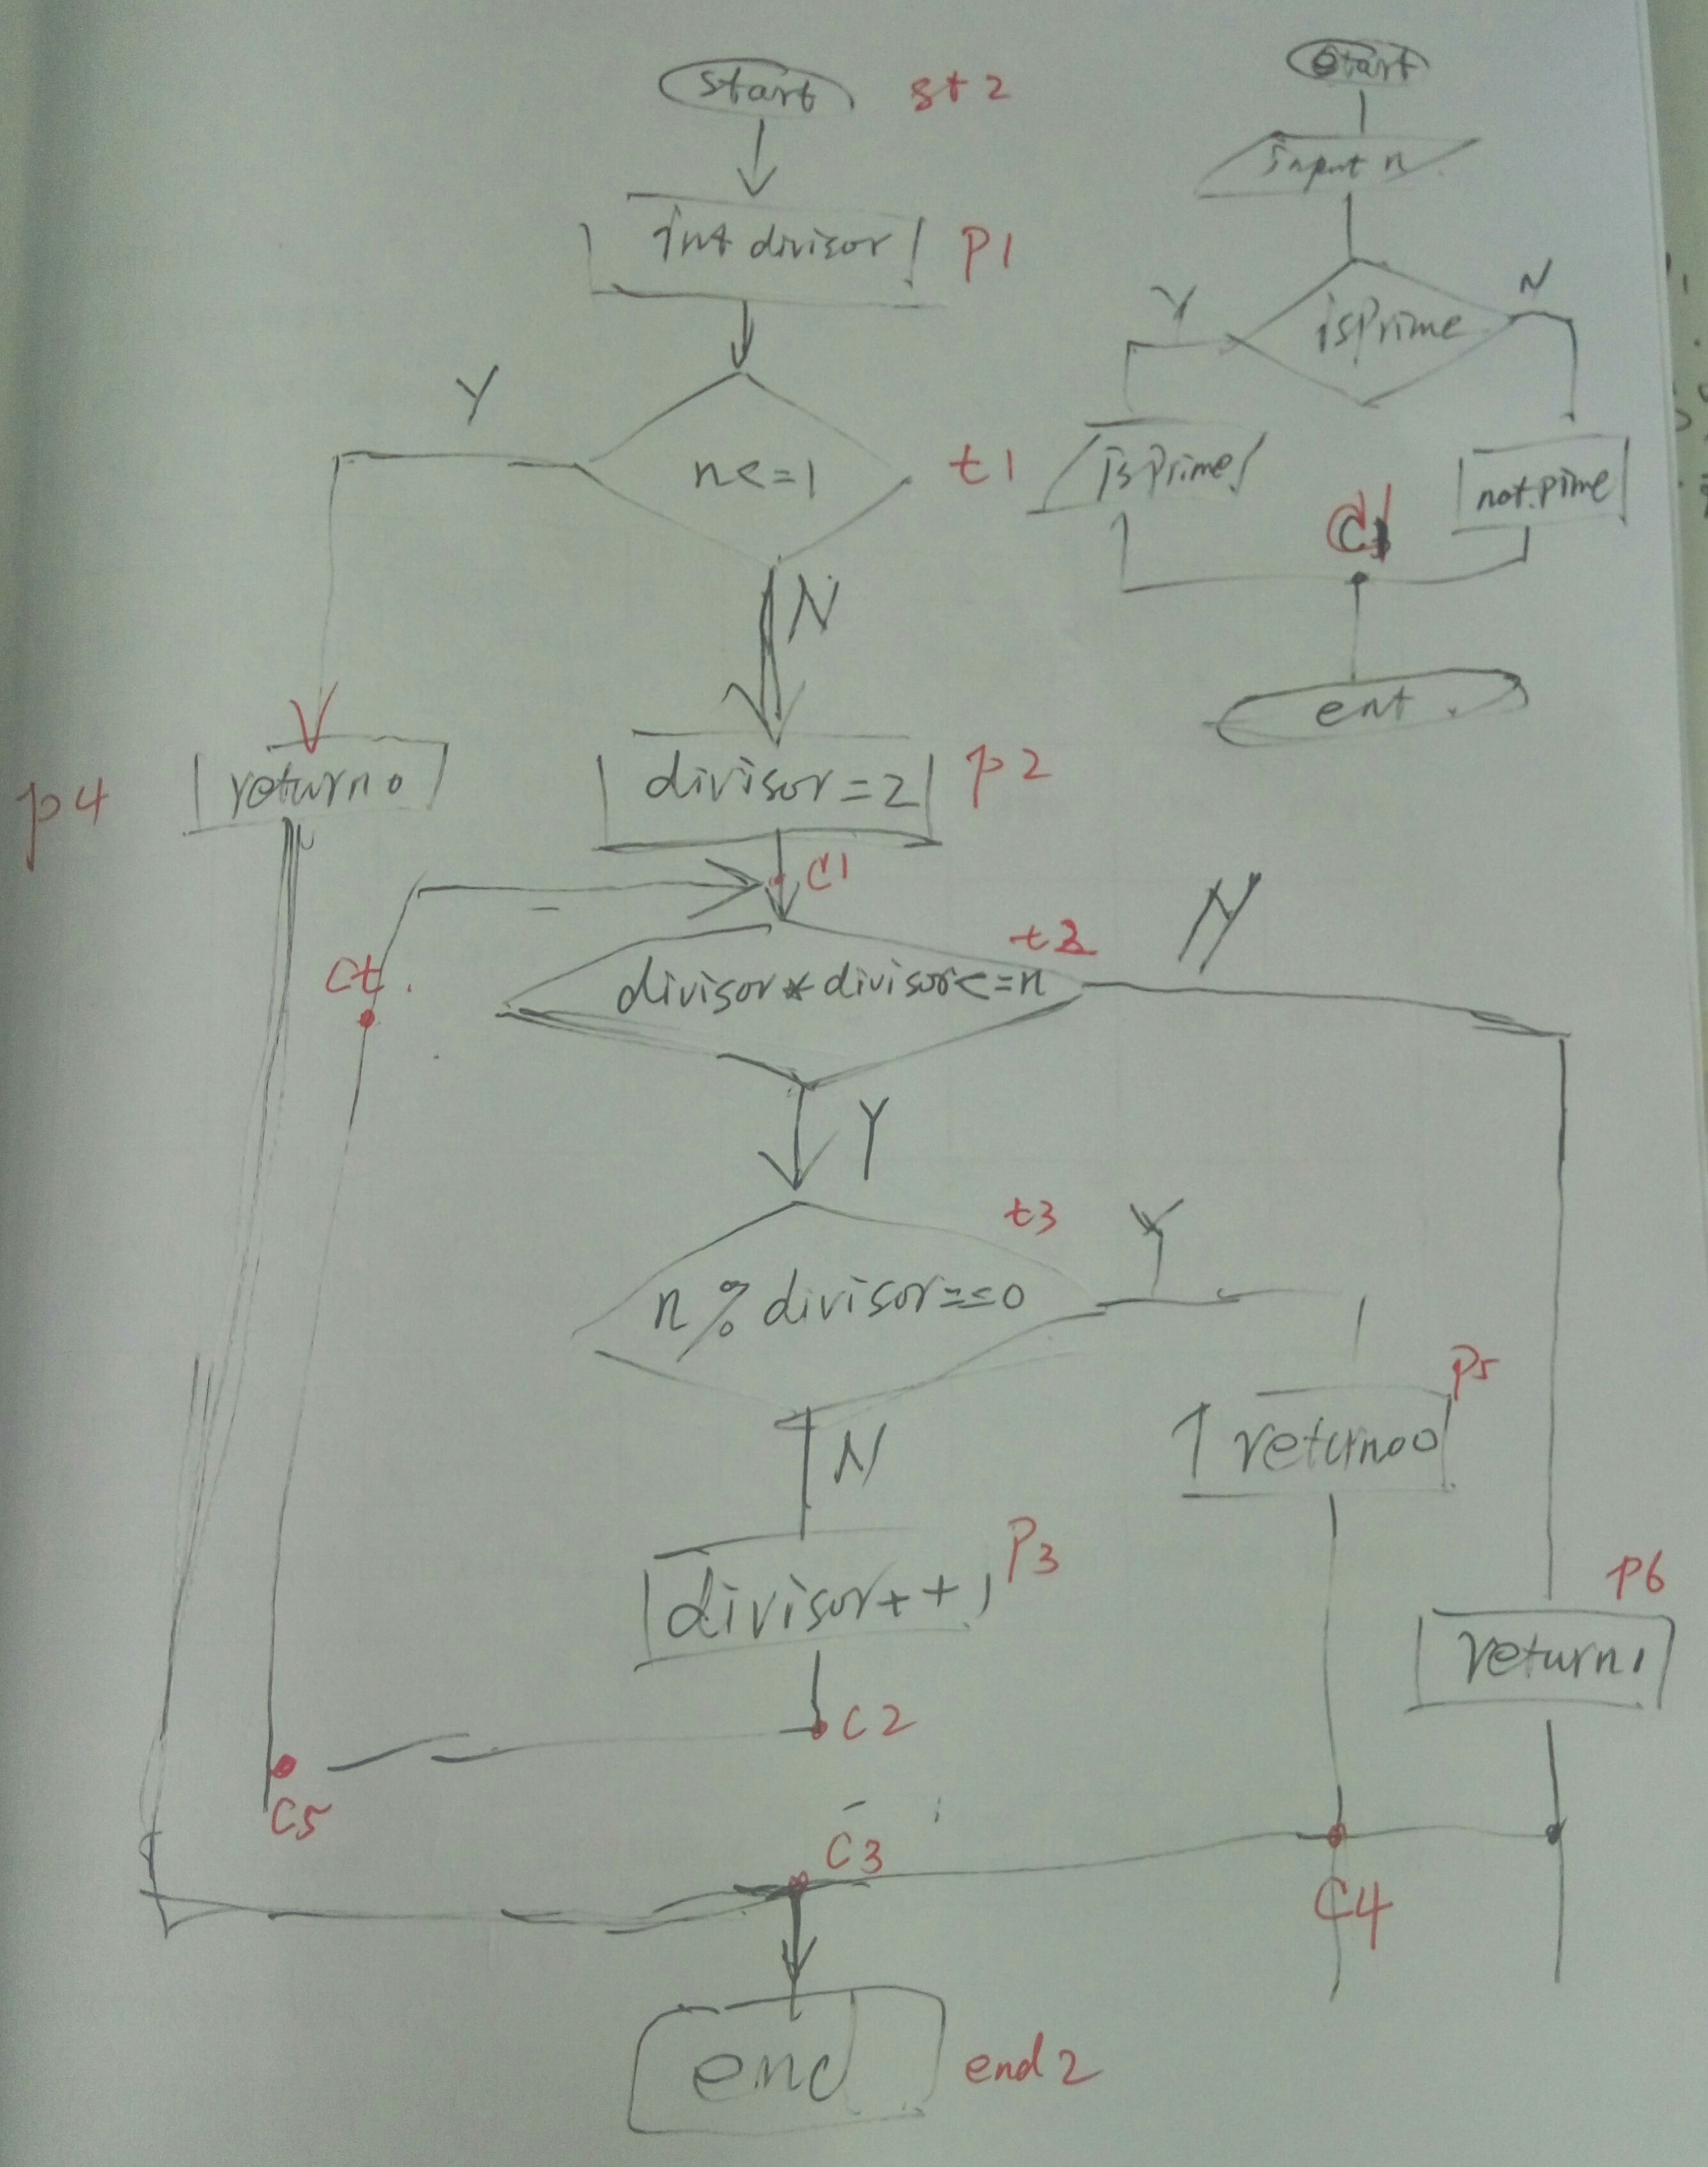
\includegraphics[width=0.35\textwidth]{02gcd}
      }{\caption{草图}\label{subfig:draft}}
      \ffigbox[\FBwidth]{
        \begin{tikzpicture}[scale=0.53,transform shape,]
          % 布置结点单元
          \node [term] (st) {开始};
          \node [proc, text width = 5em, join] (p1) {int divisor};       
          \node [test, join] (t1) {n <= 1};
          \node [proc, text width = 5em] (p2) {divisor = 2};
          \node [test, text width = 10em, join] (t2) {divisor * divisor <= n};
          \node [test, text width = 8em] (t3) {n \% divisor == 0};
          \node [proc, text width = 5em] (p3) {divisor++};
          \node [term, below = 1.6 of p3] (end) {结束};
          \node [proc, text width = 4em, left = 4.8 of t2] (p4) {return 0};
          \node [proc, text width = 4em, right = 3.5 of p3] (p5) {return 0};
          \node [proc, text width = 4em, right = 5.8 of t3] (p6) {return 1};

          % 布置用于连接的坐标结点,同时为其布置调试标记点。
          \node [coord] (c1) at ($(p2.south)!0.5!(t2.north)$)  {}; \cmark{1}
          \node [coord, below = 0.25 of p3] (c2)  {}; \cmark{2}
          \node [coord, above = 0.5 of end] (c3) {};  \cmark{3}
          \node [coord, left = 0.5 of t2] (ct) {};  \cmark{t}
          \node [coord] (c4) at (c3 -| p5)  {}; \cmark{4}
          \node [coord] (c5) at (c2 -| ct)  {}; \cmark{5}
        
          % 判断框连线,每次绘制时,先绘制一个带有一个固定
          % 位置标注的路径(path),然后再绘制箭头本身(arrow)。
          \path (t1.south) -- node [near start, right] {$N$} (p2.north);
          \draw [norm] (t1.south) -- (p2.north);
          \path (t1.west) -| node [near start, above] {$Y$} (p4.north);
          \draw [norm] (t1.west) -| (p4.north);
        
          \path (t2.south) -- node [near start, right] {$Y$} (t3.north);
          \draw [norm] (t2.south) -- (t3.north);
          \path (t2.east) -| node [near start, above] {$N$} (p6.north);
          \draw [norm] (t2.east) -| (p6.north);
        
          \path (t3.south) -- node [near start, right] {$N$} (p3.north);
          \draw [norm] (t3.south) -- (p3.north);
          \path (t3.east) -| node [near start, above] {$Y$} (p5.north);
          \draw [norm] (t3.east) -| (p5.north);

          % 其它连线
          \draw [norm](p3.south) |- (c5) |- (c1);
          \draw [norm](p4.south) |- (c3);
          \draw [norm](p4.south) |- (c3) -- (end);
          \draw [norm](p5.south) -- (c4);
          \draw [norm](p6.south) |- (c3);
          \draw [norm](p6.south) |- (c3) -- (end);
        \end{tikzpicture}
      }{\caption{TiKZ绘制图}\label{subfig:tikz}}
    \end{subfloatrow}
  }{\caption{用TiKZ绘制流程图}\label{fig:flowcharttikzdraw}}
\end{figure}

\section{标题和列表环境}
\subsection{二级标题}
\subsubsection{三级标题}
\zhlipsum[1]
\subsection{列表环境}
在\enquote{nwafucoursepaper.cls}模板中,基于enumitem宏包分别对\verb|itemize|、
\verb|enumerate|和\verb|description|三个环境的各个距离参数进行了修正,以使其排版结果
符合中文习惯的首先缩进格式。
\subsubsection{itemize环境}
\begin{itemize}
\item 床前明月光,床前明月光,床前明月光,床前明月光,床前明月光,床前明月光,床前明月光。
\item 疑是地上霜,疑是地上霜,疑是地上霜,疑是地上霜,疑是地上霜,疑是地上霜,疑是地上霜。
\item 举头望明月,举头望明月,举头望明月,举头望明月,举头望明月,举头望明月,举头望明月。
\item 低头思故乡,低头思故乡,低头思故乡,低头思故乡,低头思故乡,低头思故乡,低头思故乡。
\end{itemize}
\subsubsection{enumerate环境}
\begin{enumerate}
\item 床前明月光,床前明月光,床前明月光,床前明月光,床前明月光,床前明月光,床前明月光。
\item 疑是地上霜,疑是地上霜,疑是地上霜,疑是地上霜,疑是地上霜,疑是地上霜,疑是地上霜。
\item 举头望明月,举头望明月,举头望明月,举头望明月,举头望明月,举头望明月,举头望明月。
\item 低头思故乡,低头思故乡,低头思故乡,低头思故乡,低头思故乡,低头思故乡,低头思故乡。
\end{enumerate}
\subsubsection{description环境}
\begin{description}
\item[床前明月光],床前明月光,床前明月光,床前明月光,床前明月光,床前明月光,床前明月光。
\item[疑是地上霜],疑是地上霜,疑是地上霜,疑是地上霜,疑是地上霜,疑是地上霜,疑是地上霜。
\item[举头望明月],举头望明月,举头望明月,举头望明月,举头望明月,举头望明月,举头望明月。
\item[低头思故乡],低头思故乡,低头思故乡,低头思故乡,低头思故乡,低头思故乡,低头思故乡。
\end{description}

\section{\enquote{emph}强调字体}
在\enquote{nwafucoursepaper.cls}模板中,重定义强调字体,将默认强调字体
是italic,中文用楷体代替操作更换为加粗操作,用加粗后的字体表示强调。
\section{文本框盒子}
文本框盒子继承于自己开发的boxie宏包,其使用细节请在\github{}查看
\href{https://github.com/registor/boxiesty}{boxie宏包}的使用说明书。
同时,在该宏包的基础上,为boxie宏包添加加了摘自于
\href{https://github.com/WisdomFusion/latex-templates/tree/master/progartcn}{progartcn
  论文模板}的\enquote{标题}、\enquote{注意}、\enquote{重要}、
\enquote{技巧}和\enquote{警告}文本框环境代码\footnote{本节示例摘自于
  该模板中的tutorial-sample.tex文件}。
\subsection{\enquote{标题}文本框}
标题文本框环境的使用格式为:

\verb|\begin{titledBox}{<title>} <content> \end{titledBox}|

\begin{titledBox}{HTTP/Console 内核}
  HTTP 内核继承自 \verb|Illuminate\Foundation\Http\Kernel| 类,该类定义了一个 \verb|bootstrappers| 数组,这个数组中的类在请求被执行前运行,这些 \verb|bootstrappers| 配置了错误处理、日志、检测应用环境以及其它在请求被处理前需要执行的任务。
\end{titledBox}
\subsection{\enquote{注意}文本框}
注意文本框环境的使用格式为:

\verb|\begin{noteBox} <content> \end{noteBox}|

\begin{noteBox}
  HTTP 内核继承自 \verb|Illuminate\Foundation\Http\Kernel| 类,该类定义了一个 \verb|bootstrappers| 数组,这个数组中的类在请求被执行前运行,这些 \verb|bootstrappers| 配置了错误处理、日志、检测应用环境以及其它在请求被处理前需要执行的任务。
\end{noteBox}

\subsection{\enquote{重要}文本框}
重要文本框环境的使用格式为:

\verb|\begin{importantBox} <content> \end{importantBox}|

\begin{importantBox}
  HTTP 内核继承自 \verb|Illuminate\Foundation\Http\Kernel| 类,该类定义了一个 \verb|bootstrappers| 数组,这个数组中的类在请求被执行前运行,这些 \verb|bootstrappers| 配置了错误处理、日志、检测应用环境以及其它在请求被处理前需要执行的任务。
\end{importantBox}
\subsection{\enquote{技巧}文本框}
技巧文本框环境的使用格式为:

\verb|\begin{tipBox} <content> \end{tipBox}|

\begin{tipBox}
  HTTP 内核继承自 \verb|Illuminate\Foundation\Http\Kernel| 类,该类定义了一个 \verb|bootstrappers| 数组,这个数组中的类在请求被执行前运行,这些 \verb|bootstrappers| 配置了错误处理、日志、检测应用环境以及其它在请求被处理前需要执行的任务。
\end{tipBox}
\subsection{\enquote{警告}文本框}
警告文本框环境的使用格式为:

\verb|\begin{warningBox} <content> \end{warningBox}|

\begin{warningBox}
  HTTP 内核继承自 \verb|Illuminate\Foundation\Http\Kernel| 类,该类定义了一个 \verb|bootstrappers| 数组,这个数组中的类在请求被执行前运行,这些 \verb|bootstrappers| 配置了错误处理、日志、检测应用环境以及其它在请求被处理前需要执行的任务。
\end{warningBox}

\section{交叉引用}
在\enquote{nwafucoursepaper.cls}模板中,交叉引用基于cleveref宏包实现,
用\verb|\autoref|和\verb|\cref|命令实现引用,并对图、表、节、小节、公式、代码等引用
标记字/词进行了设置。如对一人标签为\enquote{fig:01}的图使用
\verb|\autoref{fig:01}|便可以得到\enquote{图 XX}的结果,用
\verb|\cref{texcode01}|就可以得到\enquote{代码 XX.XX}的结果。

\section{参考文献}
参考文献采用GB/T7714-2015标准的顺序编码制,使用biber+biblatex方式实现,
样式控制选择\enquote{biblatex-gb7714-2015}宏包的顺序编码制
(gb7714-2015)样式,如\cref{texcode06}:

\begin{center}
  \begin{langCVOne}[tex][texcode06][\LaTeX{}]{引用参考文献}
    % 引用参考文献
    详见文献\cite{Peebles2001-100-100}\parencite{Babu2014--}
    另见文献\cite[49]{于潇2012-1518-1523}\parencite[106]{Babu2014--}
  \end{langCVOne}
\end{center}

能够生成如下引用结果:

% 引用参考文献
详见文献\cite{Peebles2001-100-100}\parencite{Babu2014--}
另见文献\cite[49]{于潇2012-1518-1523}\parencite[106]{Babu2014--}

\section{已载入的宏包}
在\enquote{nwafucoursepaper.cls}模板中,已引入的宏包有:
\verb|etoolbox|、\verb|enumitem|、\verb|amsmath|、\verb|mathrsfs|、
\verb|amsfonts|、\verb|booktabs|、\verb|colortbl|、\verb|multirow|、
\verb|makecell|、\verb|multicol|、\verb|ulem|、\verb|biblatex|、\verb|floatrow|、
\verb|wrapfig|、\verb|boxie|、\verb|tikz-imglabels|、
\verb|tikz-flowchart|、\verb|hyperref|、\verb|cleveref|、
\verb|bookmark|、\verb|graphicx|、\verb|geometry|、
\verb|environ|、\verb|fancyhdr|、\verb|zhlineskip|、\verb|caption|,
无需再次引入这些宏包。

\section{重要文件}
\begin{importantBox}
  在使用在\enquote{nwafucoursepaper.cls}模板前请确保:
  \verb|tikz-flowchart.sty|、\verb|boxie.sty|、
  \verb|tikz-flowchart.sty|、\verb|tikz-imglabels.sty|、\verb|fvextra.sty|、\verb|lstlinebgrd.sty|这六个文件在当前
  工作文件夹中。
\end{importantBox}

% 打印参考文献表
\printbibliography[heading=bibliography,title=参考文献]
\end{document}

%%% Local Variables:
%%% mode: latex
%%% TeX-master: t
%%% End:
